\chapter{测试驱动开发} % Introduction chapter suppressed from the table of contents

\hypertarget{ux6d4bux8bd5ux9a71ux52a8ux5f00ux53d1}{%
\section{测试驱动开发}\label{ux6d4bux8bd5ux9a71ux52a8ux5f00ux53d1}}

开发人员问:为什么要这么做?写完程序后,然后再写测试用例,不是更正常吗?

\hypertarget{ux4e3aux4ec0ux4e48ux6211ux4eecux8981ux6d4bux8bd5ux9a71ux52a8ux5f00ux53d1}{%
\subsection{为什么我们要测试驱动开发}\label{ux4e3aux4ec0ux4e48ux6211ux4eecux8981ux6d4bux8bd5ux9a71ux52a8ux5f00ux53d1}}

\textbf{精益}是敏捷中很核心的概念。最近发生的一件事帮我回答了以上问题,也让我体会到TDD与精益的概念是如何协同的。

我有一位拥有三十多年电机工程经验的老同学李先生,他在对Linux的研究方面一直都很有兴趣,这几年又开始玩树莓派,目前他对此非常精通。

最近我找到他,希望在树莓派上安装 Ipython, Jupyter Notebook
等开源应用软件。一直以来,李先生的理念就是尽量用最简单、最轻易的方法去解决客户的问题,而不是浪费资源。

例如,95年开始尝试建立 wiki
服务器给客户使用的时候,他就建议我用树莓派来建:\\
他说:''树莓派不仅省电而且快,也不知道你这个概念是否持久,我不会浪费时间------在大型服务器上安装
Linux +Mediawiki ,如果你觉得这(树莓派)可以,
便继续用。如果觉得它性能不够了,下一步我帮你换更大型的服务器。''

%\href{文件:树莓派2.jpg}{300px}

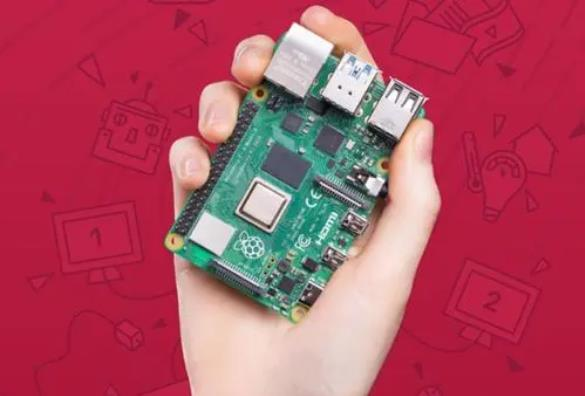
\includegraphics[width=6cm]{树莓派2.jpg}

---直到现在, 已经7
年了,我们一直还是继续用树莓派来协助评估(树莓派从原来的Pi2(1G内存),现在已经是P4(4G内存),已经服务超过百家客户了,这证明他的思路是对的。

回到我刚才说要安装 Jupyter Notebook
,他安装好那个程序包后,一直没动。我问他什么原因?他说:``
很简单,我不熟悉软件工程,也不懂如何测试。
肯定要找你测试一下,我才知道有没有做错。这样可以避免无谓的返工。''

所以我们就约好周日我回到到办公室跟他远程测试。

李先生打开树莓派后,我用VNC客户端进入他的树莓派,打一些最基本的 Ipython
指令,验证没问题。

下一步我要跑一些比较复杂的、要用到 Pandas 包的 Python
程序,却发现还没有安装Pandas包。他马上到网上去找安装介质以及树莓派如何安装
PANDAS 的方法。
处理好后,我再跑对应的程序,都跑通了,包括之前跑过的指令。前后两个小时,按本来计划,测试成功。

我回想一下,其实他的思路就是精益。用有限资源、以最低投入,达到客户要求,不多做。每当李先生做完一步,如果没有通过测试,就不会浪费时间走下一步------这也是精益和测试驱动开发的原理。

\hypertarget{ux6bcfux5c0fux6b65ux9a8cux8bc1}{%
\subsection{每小步验证}\label{ux6bcfux5c0fux6b65ux9a8cux8bc1}}

工程类的本科生都要在最后一年做毕业项目。当时,1983年,导师建议我们尝试参考一些常用的语言发声算法,在专门做信号处理的芯片上写程序,读出一些英文字或句子(与现在不同,当时这项技术还没有成熟,很多大学还在研究),虽然我预计有不小的技术难度,但觉得这很先进,很感兴趣,便与另一位同学合作,开始制定项目计划。

我们很努力,全情投入,一面要研究语言发声的算法,一面还要并行设计电子线路和软件等。我们用了
2 \textasciitilde{} 3
个月的时间做了整个电子线路板的硬件,同时还设计了整个软件架构,并使用计算机模拟,验证每个字实现算法后的发声效果,因为最后一年课程很多,时间过得很快,从9月开始准备一直到次年3月,软硬件的设计与开发终于都完成了,但是不知道什么原因就是没有声音,更不要说能读出一些字和句子了,最后项目以失败告终。

在这之前的一年,我有幸在大学的第三年进入大东电报局(Cable \&
Wireless)实习(当时香港的所有国际通讯都是经过大东),实习的部门(负责电报业务运维)正如火如荼开发一套新的电脑系统以取代本来基于UNIVAC的电报系统,总工程师让我用半年时间,在一个微机上编程,做一个系统,以从那些电脑上收集重要信息,如果发现异常就警报。头三个月都是花精力做整个系统设计,也买了一些展示电子版,准备用来展示,但由于经验不足,半年后最终什么都展示不出来。

到了2000年,在我兼读软件工程硕士课程时,开始接触到敏捷开发,才了解到两次项目失败的主因:不应该花大量时间去做前期设计------希望有一个完美的设计,而是应该一步一步迭代,先做一些最基本的简单功能,逐步优化。例如,在我的毕业项目中,应该先做出最基本的硬件、软件,起码能够发出声音,因为没有前人做过,整个项目是从未做过的实验。

敏捷大师Dave Thomas 先生在2015 演讲里提出敏捷软件开发的核心是:

\framebox{%
\begin{minipage}[t]{0.97\columnwidth}\raggedright
\begin{enumerate}
\tightlist
\item
  向你的目标迈出一小步。
\item
  从反馈调整你的理解。
\item
  重复。
\end{enumerate}

\begin{itemize}
\tightlist
\item
  当两种或以上选择的价值大致相同时,选一条让未来更容易修改(软件)的路径。
\end{itemize}\strut
\end{minipage}}


这些经历让我体会到为什么我们在写程序时,必须先想一下该怎么测试。

\hypertarget{ux7528tddux5f00ux53d1ux7a0bux5e8f}{%
\subsection{用TDD开发程序}\label{ux7528tddux5f00ux53d1ux7a0bux5e8f}}

程序员问:为什么我们要针对这么小的部分都做单元测试?

答:

\begin{enumerate}
\tightlist
\item
  小的单元测试容易写,比较简单,不会花费很多时间。
\item
  因为任何程序都会按时间变化,越来越复杂。有了单元测试,后面的测试就有依据,知道改动是否出错。没有单元测试的话,就没有信心去改程序,不知道是否没问题。
\end{enumerate}

\begin{description}
\item[]
\begin{description}
\tightlist
\item[]
(这和我们工程的概念一样,把工程细分,每个子系统都要确保质量达标,尽量找出缺陷,才进行下一步。)
\end{description}

如不相信请看附件“从 MIT OCW 学写程序”,我从头学编程的实例。如果老师没有提供单元测试和相关数据,学生写完代码后是无法验证代码是否通过,是编程的基本要求。为什么专业程序员的程序反而可以不需要先通过单元测试,写完直接便交给测试人员做系统测试?
\end{description}


网上有关于是否要TDD的争论:

\begin{itemize}
\tightlist
\item
  一派是坚持要先写测试用例,再写编码。
\item
  另一派觉得TDD太多余,如果功能测试做得全,也不一定要有单元测试。
\end{itemize}

这个争论让我想起以前教ACP敏捷管理的一个原则,叫``守 破 离''。

\hypertarget{ux5b88-ux7834-ux79bb}{%
\subsubsection{守 破 离}\label{ux5b88-ux7834-ux79bb}}

英文翻译成 ``Shu -- Ha -- Ri '' ,意思是学习合气道,要先从基本功出发
(守),按规则一步一步做。当你理解以后,就能融会贯通
(破),融合管理到一定境界就是大师级了 (离)。

像宫本武藏(江户时代著名剑术家)一样,一生赢了六十多场决斗,然而到了晚年,他在《五轮书》中总结,不要局限于某种刀法,最重要是抓住原理。

敏捷大师 Mr Cockburn 有一次到企业做 Class-responsibility-collaboration
(CRC) card 咨询培训,因为他很熟悉 CRC
方法,他觉得只要有助于面向对象设计,不一定要按原本的方式,可以简化。但学生都不熟悉,一直在问``请你告诉我们从头到尾,每一步如何做,我们照着做''大师没办法,最终按最原始的方法,一步步来教如何去做,学生才能懂,这是守破离的``守''。

TDD测试驱动开发也一样,把TDD看成``守'',当没有概念的时候,还是要从最基本的概念入手,我们每个程序都应该有测试,所以自然的顺序是先写测试用例,再写代码,这也能更好地帮助你理解程序的功能。

所以TDD就是做好程序基本功的基础,当你已经掌握这些基础了,就可以灵活处理,可能不一定要每次先写测试用例,但底线是每个代码都要有单元测试。

但是有些人觉得,只要有功能测试,单元测试可以不做。

功能测试是黑盒测试,从客户的角度测试总体功能,无法真正判断代码是否正确。反过来,单元测试是白盒测试,从代码的功能角度,验证代码是否正确,所以功能测试是不能替代单元测试的。尤其是当代码有功能上的变化时,就更需要有单元测试来验证这些改动是否有误,所以单元测试的复用率非常高。

大家正在越来越多地使用自动集成工具,如果有单元测试,那么每天的自动集成就不仅仅是看编译是否通过,还需要通过单元测试,才能更好地保证代码质量,这就是很有效率的回归测试。(回归测试:为避免因代码修改,导致原先通过的测试不通过,所以之前通过的测试用例也要重复再测。如果手工测试,为了节省测试时间,只重跑部分重要测试,但如果自动化,就可以轻松地重跑所有测试用例。)

\hypertarget{ux5355ux5143ux6d4bux8bd5ux4e0etddux7684ux597dux5904}{%
\subsection{单元测试与TDD的好处}\label{ux5355ux5143ux6d4bux8bd5ux4e0etddux7684ux597dux5904}}

上周在杭州跟一位资深的开发主管对话,他回国前在日本工作了接近10年,他说很佩服日本注重开发质量,例如很注重单元测试,所以回国后在团队严格要求要有单元测试。

我问:现在有很多静态代码检测,为何还要单元测试。

他答:目的不同,静态代码检测只是用过去的历史经验去检查常见的语法、命名问题,但如果是设计本身的逻辑问题就无法查出。
以他多年的经验,必须通过单元测试才有信心确认这个程序是否正常,单靠集成测试、功能测试是无法确保程序的每一部分都是正常的。所以他严格要求团队,代码经过检验后(自动静态检验或代码走查),还必须做单元测试才能进入下一步的集成、系统测试。

单是靠集成测试、功能测试是无法确保程序每一部分都正常。

他还说TDD 有三点好处:

\begin{enumerate}
\tightlist
\item
  让开发人员在编码前去理解设计和需求。
\item
  让开发人员知道代码可验证性的重要。
\item
  强迫开发人员主动与设计和需求人员沟通,否则无法设计出单元测试用例,但TDD
  对团队成员素质要求较高。
\end{enumerate}

\hypertarget{ux7ed3ux675fux8bed}{%
\subsection{结束语}\label{ux7ed3ux675fux8bed}}

开发人员用TDD编程,体现每走一步前必须验证通过,减少返工,精益思路,是中初级程序员健康成长之路,养成好习惯。

但若你是九段高手,因已经过了以上基本训练阶段,可能便不再需要,好比合气道``守
破 离''成长路径。

有些敏捷大师,已经累积有20年以上编程经验,例如上面提到的Thomas先生,他已经很少写单元测试,因为他觉得已经不需要依赖单元测试来验证代码是否正确。


\hypertarget{ux9644ux4ef6}{%
\section{附件}\label{ux9644ux4ef6}}

\hypertarget{ux4ece-mit-ocw-ux5b66ux5199ux7a0bux5e8f}{%
\subsection{从 MIT OCW
学写程序}\label{ux4ece-mit-ocw-ux5b66ux5199ux7a0bux5e8f}}

第四天早上10:00我终于把所有功能写完并通过自动单元测试!\\
(趁十一长假做编码练习题。上次做题已经是春节后,在集中隔离期间做过两题。这次的练习题只有十个功能,本来预计可两天完成。)

\framebox{%
\begin{minipage}[t]{0.97\columnwidth}\raggedright
练习题 (Problem
Set)------分析美国过去温度变化,提供了美国超过20个城市的每天平均温度。(从1961年到2015年)

\begin{itemize}
\tightlist
\item
  先写基本功能:

  \begin{itemize}
  \tightlist
  \item
    画散点图,回归分析,计算标准差与决定系数 (R\textsuperscript{2} Coef.
    of determination)
  \end{itemize}
\end{itemize}

\begin{itemize}
\tightlist
\item
  分析过去的五六十年数据,来判断美国或全球是否在暖化
\end{itemize}

给学生的文件包:

\begin{enumerate}
\tightlist
\item
  ProblemSet5.pdf : 分成 A、 B 、C、 D、
  E部分,详细说明每部分要开发的功能
\item
  PS5.py 程序模板,学员填入代码
\item
  PS5\_test.py 自动单元测试模块,自动测写好的PS5.py
\end{enumerate}\strut
\end{minipage}}


回顾一下,像我这种Python新手,因为不熟悉Python语言的属性与特性,必须按部就班,一步一步来写,欲速则不达。

更重要是体会到个人如何记录数据并分析:

\framebox{%
\begin{minipage}[t]{0.97\columnwidth}\raggedright
\hypertarget{ux8bb0ux5f55ux65f6ux95f4}{%
\subsubsection{记录时间}\label{ux8bb0ux5f55ux65f6ux95f4}}

十多年前我在美国考CMMI培训师,被观察时,
观察老师会在培训后告诉我,每一个模块用了多少时间,与计划对比。
从此以后每次培训我都会习惯记录每个模块所花的时间。

\hypertarget{ux600eux6837ux505a}{%
\subsubsection{怎样做}\label{ux600eux6837ux505a}}

培训时,我都会在桌上放一数字电子钟,记录每一个模块的开始时间与结束时间。上完一天课,晚上在电子表单计划时间旁边写上每个模块的实际时间。
这三天半,我也是用这种方式记录每个模块的时间。

\hypertarget{ux8bb0ux5f55ux7f3aux9677}{%
\subsubsection{记录缺陷}\label{ux8bb0ux5f55ux7f3aux9677}}

因为每个功能都很小,不到20行, 所以没有正式把缺陷与返工工作量记下来。
尤其是一些小的语法错误问题立马就改正了。
但影响较大的重大缺陷,我会记在模块旁边,算是这个模块花的时间。

个人记录实际时间没有想象中这么困难,
只要每天晚上简单按当天本子的数据更新电子表单,避免遗忘。

%\href{文件:PspLogScreenshot20211006174917.png}{500px}
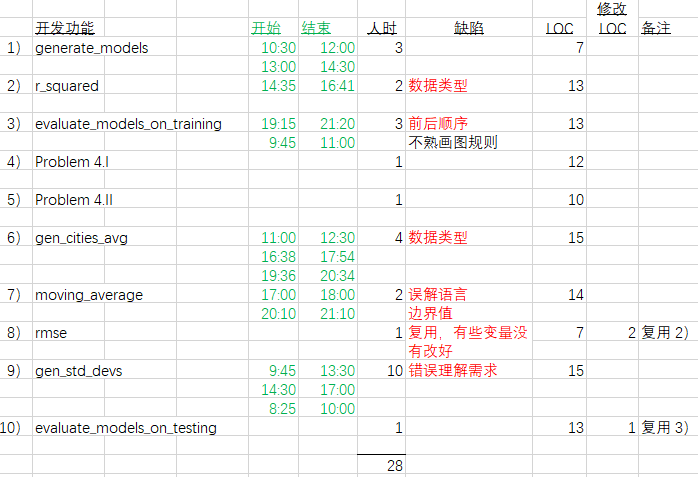
\includegraphics[width=6cm]{PspLogScreenshot20211006174917.png}

\strut
\end{minipage}}


\hypertarget{ux56deux987eux5206ux6790}{%
\subsubsection{回顾分析}\label{ux56deux987eux5206ux6790}}

整个编程结束后,写上每一个模块的实际代码行数。注意:如果模块是复用其他模块代码,便需要注明改动的代码行数。例如:evaluate\_models\_on\_testing13行只修改了1行。

分析:除了标准差模块(gen\_std\_devs)以外,其他功能都能在1-3个小时之内完成。

计算标准差的功能花了 10
小时,问题出在我编码时没有详细看需求。开始以为是求每个城市的温度标准差。
然后再求标准差的平均数。\\
测试不通过后,
也没有再看需求便假定求当年几个城市所有当年每天温度的标准差,还是不对。
到了第四天早上再看看 ProblemSet5.pdf
需求描述才知道我一直误解了这功能需求。

\framebox{%
\begin{minipage}[t]{0.97\columnwidth}\raggedright
gen\_std\_devs对应每一输入年份,返回一个数值,依据以下计算:\\ 1)按输入的所有城市,计算当年每一天的平均温度(所有城市的平均)\\ 
2)计算当年每一天平均温度的标准差\strut
\end{minipage}}


所以如按我本来的算法,算一个城市是正确,但两个或者多个城市的时候,答案就比正确答案大。

针对这个计算标准差问题,一直以为是语法问题公式计算错误问题。
但我用一些简单的数据检验去,未能发现任何不正常。
来来去去都没有实际的进展,差点想放弃。

\framebox{%
\begin{minipage}[t]{0.97\columnwidth}\raggedright
经验教训

\begin{itemize}
\tightlist
\item
  最佳实践: 尽量用最小的行数完成功能

  \begin{itemize}
  \tightlist
  \item
    像Python这类成熟的语言,绝大部分的功能都已经具备
  \item
    尽量避免基础方法编写一个已有的功能(reinvent the
    wheel),除了耗费时间外,还会写多错多
  \end{itemize}
\end{itemize}

\begin{itemize}
\tightlist
\item
  写任何程序前必须先有自动化测试用例

  \begin{itemize}
  \tightlist
  \item
    虽然自己可以先想一些数据自己简单测一下
  \item
    但替代不了另外一个人写的测试用例。跑通才有信心程序正确
    (所以自动单元测试是使用最多的程序)
  \end{itemize}
\end{itemize}

\begin{itemize}
\tightlist
\item
  架构与设计很重要

  \begin{itemize}
  \tightlist
  \item
    校方除了提供测试脚本外,还提供了写程序的模板 (PS5.py)
  \item
    每个功能都明确,输入是什么,什么数据类型,输出是什么
  \item
    学员自己只需要填写实现的代码部分
  \end{itemize}
\end{itemize}

\begin{itemize}
\tightlist
\item
  先把握好新功能的用法与结果

  \begin{itemize}
  \tightlist
  \item
    前面发现不少缺陷,是因为不清楚某功能的用法
  \item
    在写代码之前,自己应开个沙盘,用小程序先试验一下这计算功能有什么参数,会出什么结果
  \end{itemize}
\end{itemize}

\begin{itemize}
\tightlist
\item
  先评审后测试

  \begin{itemize}
  \tightlist
  \item
    在跑程序之前,屏幕展示或打印出刚写好的代码,用铅笔在白纸上按程序的逻辑,从头思考一下每个数据的种类和中间的变化
  \item
    盲目地去跑程序或测试,最终只得出测试失败,但还不清楚错在哪里,如何修改。所以不如在跑程序或测试前,自己先动脑筋模拟一次,仔细想通每个数据的变化
  \end{itemize}
\end{itemize}\strut
\end{minipage}}





